\documentclass[10pt,a4paper]{article}
\usepackage[margin=2cm,top=1.8cm,bottom=1.8cm]{geometry}
\usepackage[T1]{fontenc}\usepackage{lmodern}\usepackage{microtype}
\usepackage{graphicx,booktabs,caption,tikz,float}
\usetikzlibrary{arrows.meta,positioning,shapes.misc,calc}
\captionsetup{font=small,labelfont=bf,skip=4pt}
\usepackage[hidelinks]{hyperref}
\setlength{\parskip}{2pt}\setlength{\parindent}{1em}
\usepackage{titlesec}\titlespacing*{\section}{0pt}{8pt}{3pt}\titlespacing*{\subsection}{0pt}{5pt}{2pt}
\titleformat{\section}{\normalfont\large\bfseries}{\thesection}{0.6em}{}
\titleformat{\subsection}{\normalfont\normalsize\bfseries}{\thesubsection}{0.6em}{}
\graphicspath{{figures/}}
\title{\vspace{-1.2cm}\Large A large language model as one replanning strategy inside a MATSim population:\\the first complete campaign run}
\author{\normalsize Giulio Iannelli \quad MATSim AI Lab \quad \texttt{matsim-ai-lab}, branch \texttt{migrate/contrib-llm}, commit \texttt{a916897}}
\date{\normalsize 24 September 2026}
\begin{document}\maketitle\vspace{-0.9cm}

\begin{abstract}\noindent
MATSim simulates a city day by day: every synthetic traveller carries a few daily plans, executes one, is scored on it, and occasionally changes it with a rule-based strategy until the population settles. We replace that strategy, for a panel of 200 travellers out of 8,460, by a local 27-billion-parameter language model that reads the day in the first person and decides per trip which mode to use. This report documents the first complete run of this set-up: 25 iterations, 10 model queries per iteration, 3\,h\,06\,min on a shared GPU server. All 250 queries produced a valid decision in a single model round (median 39\,s). The model changed 59 of 250 days, almost always from public transport to car, citing transfers and age. MATSim's scoring kept those changes for 15 of the 42 travellers concerned and discarded the plan outright for 16. The population as a whole did not move. A context bug found in the first attempt, which silently forbade every car switch, is reported because it changes how vehicle availability must be presented to a language model.
\end{abstract}

\section{Question and setting}
MATSim is an agent-based transport simulation. Each agent owns up to six daily plans (a chain of activities with trips between them). In every iteration one plan per agent is executed on the road and transit network, scored with a utility function (time at activities is rewarded, travel time and cost are penalised), and a fraction of agents replan: a copy of a plan is modified by a \emph{strategy} (re-route, shift departure times, change mode) while the rest keep the plan with the best score. Over many iterations the population relaxes to a user equilibrium.

The question of this work is whether a language model (LLM) can act as one of these strategies for a subset of agents, so that mode decisions are made by a persona with stated age, job and car access instead of by random mutation, while MATSim keeps the final word through scoring. Two things must hold for that to be a usable research instrument: the protocol must be reliable (every query yields a plan MATSim can run) and fast enough that a run with hundreds of queries fits in an afternoon. Only then do the decisions themselves become worth analysing. This report measures both, on the first run that completed.

\section{Method}
\subsection{Ground}
Scenario: Sioux Falls, the standard MATSim test city (car, bus, walk). A 10\,\% sample of the population (8,460 agents) with road and transit capacities scaled to 0.1 was run for 100 rule-based iterations beforehand. The resulting plans are the \emph{warmed ground}: mean executed score 18.76\,$\rightarrow$\,20.16, mode shares car/pt/walk 78/19/3\,\% $\rightarrow$ 61/28/11\,\%, no agent stuck in traffic. Every LLM run starts from these plans, so the population is already at rest and any drift is caused by the LLM.

\subsection{Panel and trigger}
A seeded panel of 200 agents is tagged. In each iteration at most 10 of them are handed to the LLM; the others, and the 8,260 agents outside the panel, replan with MATSim's default strategies. Priority: agents that got stuck, then agents never reviewed, then the 20\,\% of the panel with the worst drop of executed score since their last review. With 200 agents and 10 per iteration, the first 20 iterations review everyone once; from iteration 21 the score-drop trigger drives selection.

\subsection{One query, one round}
Earlier runs let the model call tools (route, compare modes, list available modes) over 6--9 rounds per agent, 375\,s each. Here the facts are pre-computed and written into the first message: the activity chain; which vehicles the agent owns and where each is parked at the start of the day; and for every trip the travel time, distance and transfers by car, bus and walk from MATSim's own router on today's congested network. The model answers with one tool call, \texttt{decide\_trips}: a list of trips to change, each with a new mode and an optional departure shift (empty list = keep the day). The decision is checked (trip exists, mode known, the vehicle is actually with the traveller along the chain of trips), then MATSim routes the new legs. Prompt: 2,673 tokens median; answer: 745 tokens median, of which almost all is the model's reasoning trace.

\subsection{Model and prompt}
qwen3.6:27b served by Ollama on a shared GPU server (one request at a time), temperature 0.3, context 12,288 tokens, hard cap of 3,072 output tokens per round, model kept resident 10\,min between calls. The system prompt puts the model in the first person (``You are a 53-year-old man. You work. You have a car you can use whenever you want.''), states MATSim's physical rules (a vehicle moves with you; driving out and back is fine, bus out and driving back is not), and asks for short reasoning. The user message carries the plan and the pre-computed facts.

\begin{figure}[t]\centering\small
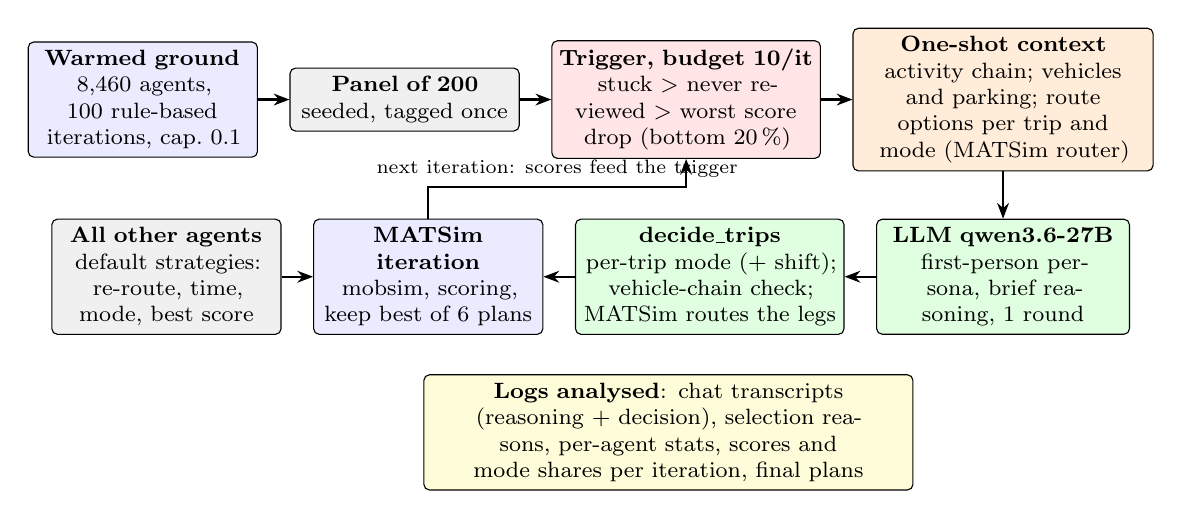
\begin{tikzpicture}[node distance=3mm and 4mm, font=\footnotesize,
  box/.style={draw, rounded corners=2pt, align=center, inner sep=3pt, minimum height=8mm, fill=#1},
  arr/.style={-{Stealth[length=2mm]}, thick}]
\node[box=blue!8, text width=27mm] (ground) {\textbf{Warmed ground}\\8,460 agents, 100 rule-based iterations, cap.\ 0.1};
\node[box=gray!12, text width=27mm, right=of ground] (panel) {\textbf{Panel of 200}\\seeded, tagged once};
\node[box=red!10, text width=32mm, right=of panel] (trig) {\textbf{Trigger, budget 10/it}\\stuck $>$ never reviewed $>$ worst score drop (bottom 20\,\%)};
\node[box=orange!15, text width=36mm, right=of trig] (ctx) {\textbf{One-shot context}\\activity chain; vehicles and parking; route options per trip and mode (MATSim router)};
\node[box=green!12, text width=30mm, below=6mm of ctx] (llm) {\textbf{LLM qwen3.6-27B}\\first-person persona, brief reasoning, 1 round};
\node[box=green!12, text width=32mm, left=of llm] (dec) {\textbf{decide\_trips}\\per-trip mode (+ shift); vehicle-chain check; MATSim routes the legs};
\node[box=blue!8, text width=27mm, left=of dec] (sim) {\textbf{MATSim iteration}\\mobsim, scoring, keep best of 6 plans};
\node[box=gray!12, text width=27mm, left=of sim] (rest) {\textbf{All other agents}\\default strategies: re-route, time, mode, best score};
\node[box=yellow!15, text width=60mm, below=5mm of sim.south west, anchor=north west, xshift=14mm] (log) {\textbf{Logs analysed}: chat transcripts (reasoning + decision), selection reasons, per-agent stats, scores and mode shares per iteration, final plans};
\draw[arr] (ground) -- (panel); \draw[arr] (panel) -- (trig); \draw[arr] (trig) -- (ctx); \draw[arr] (ctx) -- (llm); \draw[arr] (llm) -- (dec); \draw[arr] (dec) -- (sim);
\draw[arr] (rest) -- (sim);
\draw[arr] (sim.north) -- ++(0,4mm) -| node[pos=0.25, above, font=\scriptsize]{next iteration: scores feed the trigger} (trig.south);
\end{tikzpicture}
\caption{The loop. Ten panel agents per iteration are decided by the LLM; everyone else replans with MATSim's rules. Scoring is the same for all plans, so an LLM plan survives only if it scores well.}
\label{fig:scheme}
\end{figure}

\subsection{Run}
25 iterations, seed 4721, launched 16:30 and finished 19:36 on 23 September 2026. Iteration 0 executes the ground without replanning. Innovation was never switched off, so the LLM was queried in all 25 replanning iterations. Everything below comes from the run's own logs (the analysis script and numbers are in \texttt{research/persona-emergence/paper/}).

\section{Results}
\subsection{Protocol and speed}
\begin{table}[h]\centering\small
\begin{tabular}{lrlr}\toprule
queries & 250 & decisions applied by MATSim & 250 \\
model rounds per query & 1 (all) & retries / verification failures / cap hits & 0 / 0 / 0 \\
wall time per query, median (max) & 39\,s (105\,s) & model resident / after a reload & 32\,s / 52\,s \\
LLM time: generation / prompt / load & 66 / 8 / 25\,\% & generation speed & 26 tokens/s \\
run wall time & 186\,min & iteration, median (min--max) & 6.4\,min (5.4--9.7) \\
\bottomrule\end{tabular}
\caption{Protocol and timing of the run.}\label{tab:protocol}\end{table}

Every query ended with a valid decision in the first model round; no agent had to be re-asked and no decision was rejected by the chain check (Table~\ref{tab:protocol}). The distribution of query times is bimodal (Fig.~\ref{fig:timing}b): 32\,s when the model is resident on the GPU, 52\,s when it has to be reloaded first. The reloads are not ours. A colleague ran the same model on the same server with a smaller context window during iterations 1--3 and 17--25, and Ollama reloads the 17\,GB weights on every switch (Fig.~\ref{fig:timing}a, \ref{fig:iterations}). Reload-free iterations take 5.5\,min, of which about 5.3\,min are the ten LLM queries and 30\,s is MATSim itself; with the colleague active an iteration takes 9\,min. A quarter of the whole run was spent reloading.

\begin{figure}[h]\centering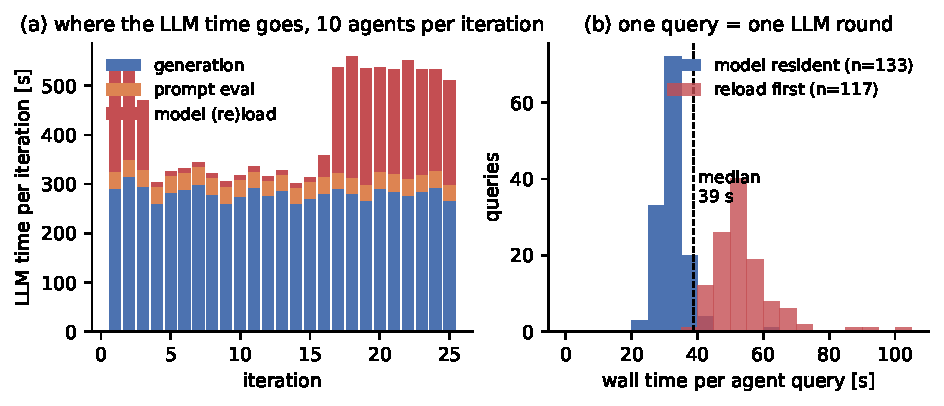
\includegraphics[width=0.9\textwidth]{fig_timing}
\caption{LLM time. (a) Per iteration, split into generation, prompt evaluation and model loading. (b) Wall time per query.}\label{fig:timing}\end{figure}
\begin{figure}[h]\centering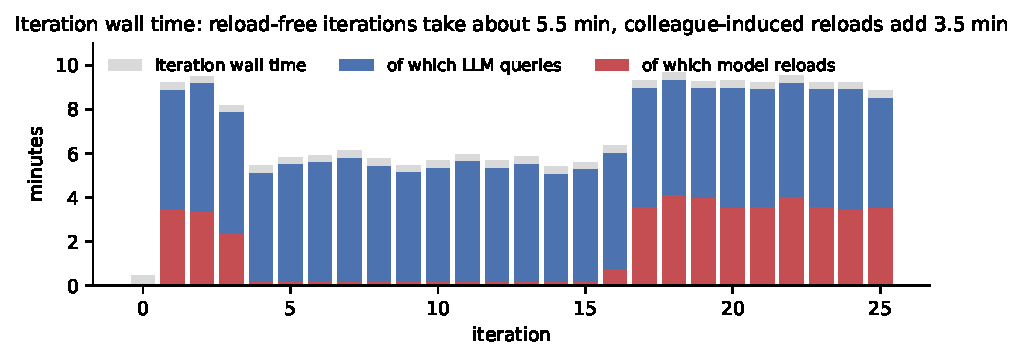
\includegraphics[width=0.9\textwidth]{fig_iterations}
\caption{Iteration wall time. Grey: whole iteration; blue: the ten LLM queries; red: the part of those queries spent reloading the model after another user's job.}\label{fig:iterations}\end{figure}

\subsection{What the model decided}
The model kept the day unchanged in 191 of 250 queries and changed at least one trip in 59, involving 42 distinct agents (Fig.~\ref{fig:decisions}a). Changes are almost entirely one kind: 102 of 113 changed trips became car trips, 4 became bus, 7 walk; no departure time was shifted (Fig.~\ref{fig:decisions}b). The typical reasoning is a car owner whose surveyed plan uses the bus with two to four transfers: ``Four transfers each way? At 53, I don't want to be hopping on and off multiple lines just to get to work.'' The model switches to car out and back even where the pre-computed car time is longer than the bus time. Agents without a car keep the bus and reject walking on distance and age; nobody proposed a car they did not own.

\begin{figure}[h]\centering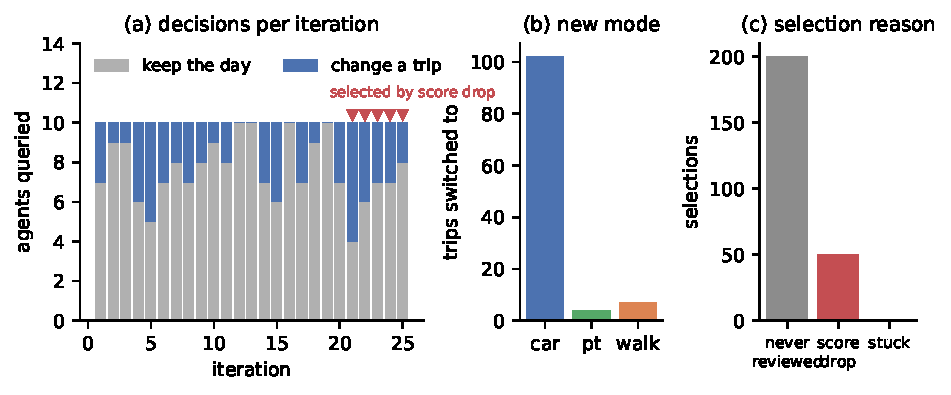
\includegraphics[width=0.9\textwidth]{fig_decisions}
\caption{Decisions. (a) Keep versus change per iteration; red markers: iterations in which agents were selected by score drop. (b) New mode of the 113 changed trips. (c) Why agents were selected.}\label{fig:decisions}\end{figure}

\subsection{Panel dynamics}
Iterations 1--20 reviewed all 200 panel agents once (Fig.~\ref{fig:decisions}c). From iteration 21 the trigger selected 50 agents by executed-score drop (median drop 0.22 utils, maximum 4.25); 39 agents were therefore queried twice or more. Their second answers are consistent with their first: all 17 agents that had changed a trip changed it again (15 to car again), and 32 of 33 that had kept their day kept it again. The persona is stable across iterations; it does not learn from the score, because the prompt does not show it.

\subsection{The population did not move}
Mean executed score went from 20.157 to 20.166 over 25 iterations; the best and worst plans moved by less than 0.05; mode shares changed by under one point (car 61.1\,$\rightarrow$\,60.2\,\%, bus 27.6\,$\rightarrow$\,28.0\,\%, walk 11.3\,$\rightarrow$\,11.7\,\%); no agent was stuck at the end (Fig.~\ref{fig:ground}). Ten LLM decisions per iteration among 8,460 agents are invisible at population level, which is what a controlled experiment needs: the LLM's effect can be read per agent without confounding from a drifting ground.

\begin{figure}[h]\centering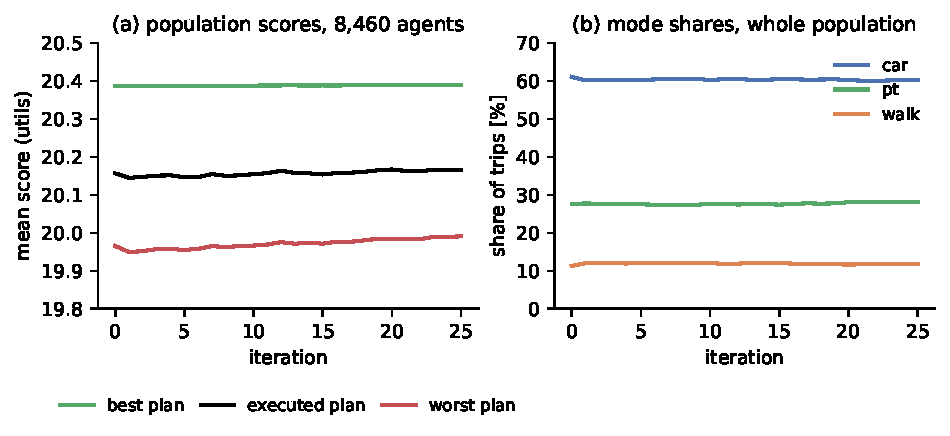
\includegraphics[width=0.86\textwidth]{fig_ground}
\caption{Ground health over the run. (a) Mean score of the executed, best and worst plan. (b) Mode shares of all trips.}\label{fig:ground}\end{figure}

\subsection{Did the LLM's plans survive scoring?}
For the 42 agents whose day the model changed, the final plan memory was inspected (Fig.~\ref{fig:survival}a). For 16 of them no plan with the LLM's modes exists any more: it scored worst among the agent's six plans and MATSim removed it. For 26 the LLM plan is still in memory, and for 15 it is the best-scoring plan and the one executed at the end. Among the 24 agents that hold both an LLM-mode plan and an alternative, the score difference is small: median $+0.05$ utils, 20 of 24 within $\pm0.5$ (Fig.~\ref{fig:survival}b). The picture is therefore not ``car always loses'': under capacity 0.1 the car and bus plans of these commuters score about the same, and MATSim's selection is close to a coin toss between them, while a clear minority of switches (the 16 dropped plans) were plainly worse. This is the first quantitative reading of how often persona preference and the utility function disagree.

\begin{figure}[h]\centering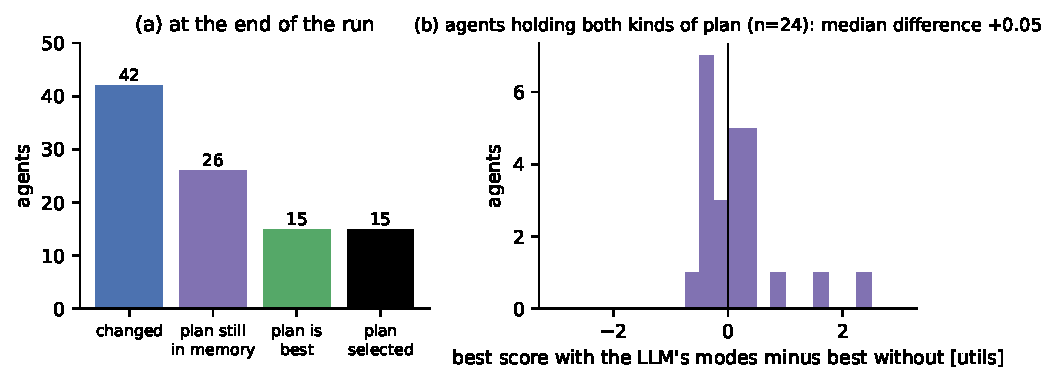
\includegraphics[width=0.9\textwidth]{fig_survival}
\caption{Fate of the 42 changed days at the end of the run. (a) How many still hold a plan with the LLM's modes, have it as their best plan, and execute it. (b) Score of the best plan with the LLM's modes minus the best plan without, for agents holding both.}\label{fig:survival}\end{figure}

\subsection{Persona}
With the short-reasoning instruction the traces still speak in the first person: median 3.4 first-person markers per 100 words, and the automatic detector counts the persona as ``emerged'' (first-person voice plus at least two grounded traits) in 195 of 250 conversations (Fig.~\ref{fig:persona}). Age is cited in 241 conversations, car ownership in 197, employment in 52. No degenerate repetition loops and no contradiction between a stated trait and a decision (for example a carless agent choosing car) were detected.

\begin{figure}[h]\centering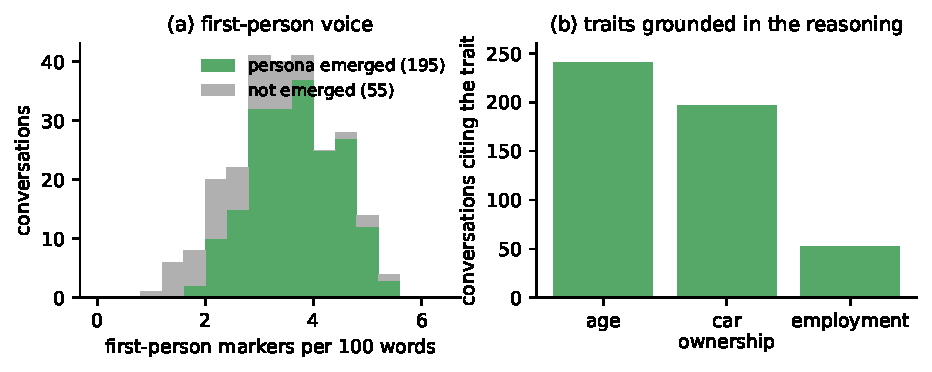
\includegraphics[width=0.86\textwidth]{fig_persona}
\caption{Persona signals in the reasoning traces. (a) First-person density, split by whether the detector counts the persona as emerged. (b) Traits cited.}\label{fig:persona}\end{figure}

\section{A bug that looked like a result}
The first attempt at this run was stopped after two iterations: 23 of 24 decisions were ``keep'', and the traces showed why. The context listed the modes available \emph{at each place under the current plan}. A car owner who commutes by bus has the car at home, so the list said ``from work: walk, bus, passenger'' and the return trip had no car option. Together with the rule ``the car is wherever you last parked it'', the model concluded it could not drive home and therefore did not drive out either; three agents said so explicitly. The population the panel is meant to move, car owners on a bad bus connection, was exactly the one the context immobilised.

The fix presents vehicles at the level of the whole day: where the car is parked in the morning, and for every trip the car option with the condition ``requires driving trip 1 as well'' where a chain is needed. The decision check follows the same chain. On the same ten agents (same seed) the change count went from 0 to 3, all car out and back (Fig.~\ref{fig:fix}). The lesson generalises: any fact given to a language model that is conditional on the plan being changed must be stated as a conditional, or the model will read it as a constraint.

\begin{figure}[H]\centering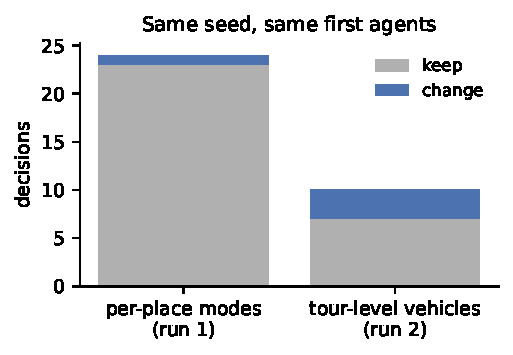
\includegraphics[width=0.4\textwidth]{fig_context_fix}
\caption{Same seed and first agents, before and after the context fix.}\label{fig:fix}\end{figure}

\section{Limitations and next steps}
One seed, one model, one city, ten queries per iteration: the numbers above characterise the instrument, not the phenomenon. Three things are missing before the scoring verdict can be interpreted. (i) A rule-based control: the same panel and trigger, with MATSim's mode-choice strategy in place of the LLM, to see how often \emph{its} changes survive. (ii) A per-agent decision table across iterations (decision, score before and after, fate of the plan) as a standard analysis command, replacing the ad-hoc script used here. (iii) Feedback: the agent is told nothing about how its last plan scored, so the 17 re-selected changers simply repeat themselves; giving the persona its own experience is the point of the memory work planned next. On the engineering side, the only remaining speed lever is to run the MATSim side on the GPU server as well, so that a run no longer depends on a laptop staying open, and to shield the run from other users' model switches.

\end{document}
